\subsection{Les filtres}
\label{sec:filtres}

Dans la théorie du contrôle, les filtres sont utilisés pour améliorer la qualité des mesures issues des capteurs avant qu'elles ne soient exploitées par le contrôleur. Les mesures réelles sont en effet souvent perturbées par du bruit, des parasites ou des variations rapides qui peuvent dégrader les performances d'un système asservi. Un filtrage approprié permet de réduire ces perturbations tout en conservant les informations utiles au contrôle. \\

L'étude des filtres repose sur deux outils fondamentaux de l'automatique : le domaine de Laplace et la fonction de transfert. Ces outils permettent de décrire mathématiquement le comportement dynamique d'un système de manière beaucoup plus simple que les équations différentielles utilisées dans le domaine temporel. \\

\paragraph{Domaine de Laplace}

Dans le domaine temporel, le comportement d'un système est généralement décrit par une équation différentielle. Par exemple, un filtre passe-bas du premier ordre peut être représenté par une équation faisant intervenir la dérivée de la sortie par rapport au temps. 

Manipuler directement ces équations devient rapidement complexe lorsque les systèmes possèdent plusieurs états ou plusieurs dérivées. Afin de simplifier leur étude, on utilise la transformée de Laplace, qui convertit les équations différentielles en équations algébriques.

La transformée de Laplace d'un signal $x(t)$ est définie par :
\begin{equation}
    X(s) = \mathcal{L}\{x(t)\} = \int_{0}^{\infty} x(t) e^{-st} dt
\end{equation}

où $s = \sigma + j\omega$ est une variable complexe composée de :
\begin{itemize}
    \item $\sigma$, qui traduit l'amortissement ou la croissance du signal
    \item $\omega$, qui représente la fréquence du signal en radians par seconde
\end{itemize}

L'un des principaux intérêts de cette transformation est que les dérivées deviennent de simples multiplications par $s$. Ainsi, 
\begin{equation}
    \frac{d}{dt} \longrightarrow s
\end{equation}

Cette propriété simplifie considérablement l'étude des systèmes dynamiques et permet notamment d'analyser leur stabilité, leur 
rapidité ainsi que leur comportement en fréquence. \\

\paragraph{Fonction de transfert}

Une fois le système exprimé dans le domaine de Laplace, il est possible de définir sa fonction de transfert. La fonction de transfert 
représente le rapport entre la sortie et l'entrée du système :
\begin{equation}
    H(s) = \frac{Y(s)}{X(s)}
\end{equation}

où :
\begin{itemize}
    \item $X(s)$ est la transformée de Laplace du signal d'entrée
    \item $Y(s)$ est la transformée de Laplace du signal de sortie
\end{itemize}

La fonction de transfert caractérise complètement le comportement dynamique d'un système linéaire lorsque les conditions initiales sont nulles. 
Elle permet notamment de déterminer la stabilité d'un système, sa rapidité de réponse ainsi que son comportement vis-à-vis des différentes 
fréquences présentes dans un signal.

\begin{sidewaysfigure}
    \centering
    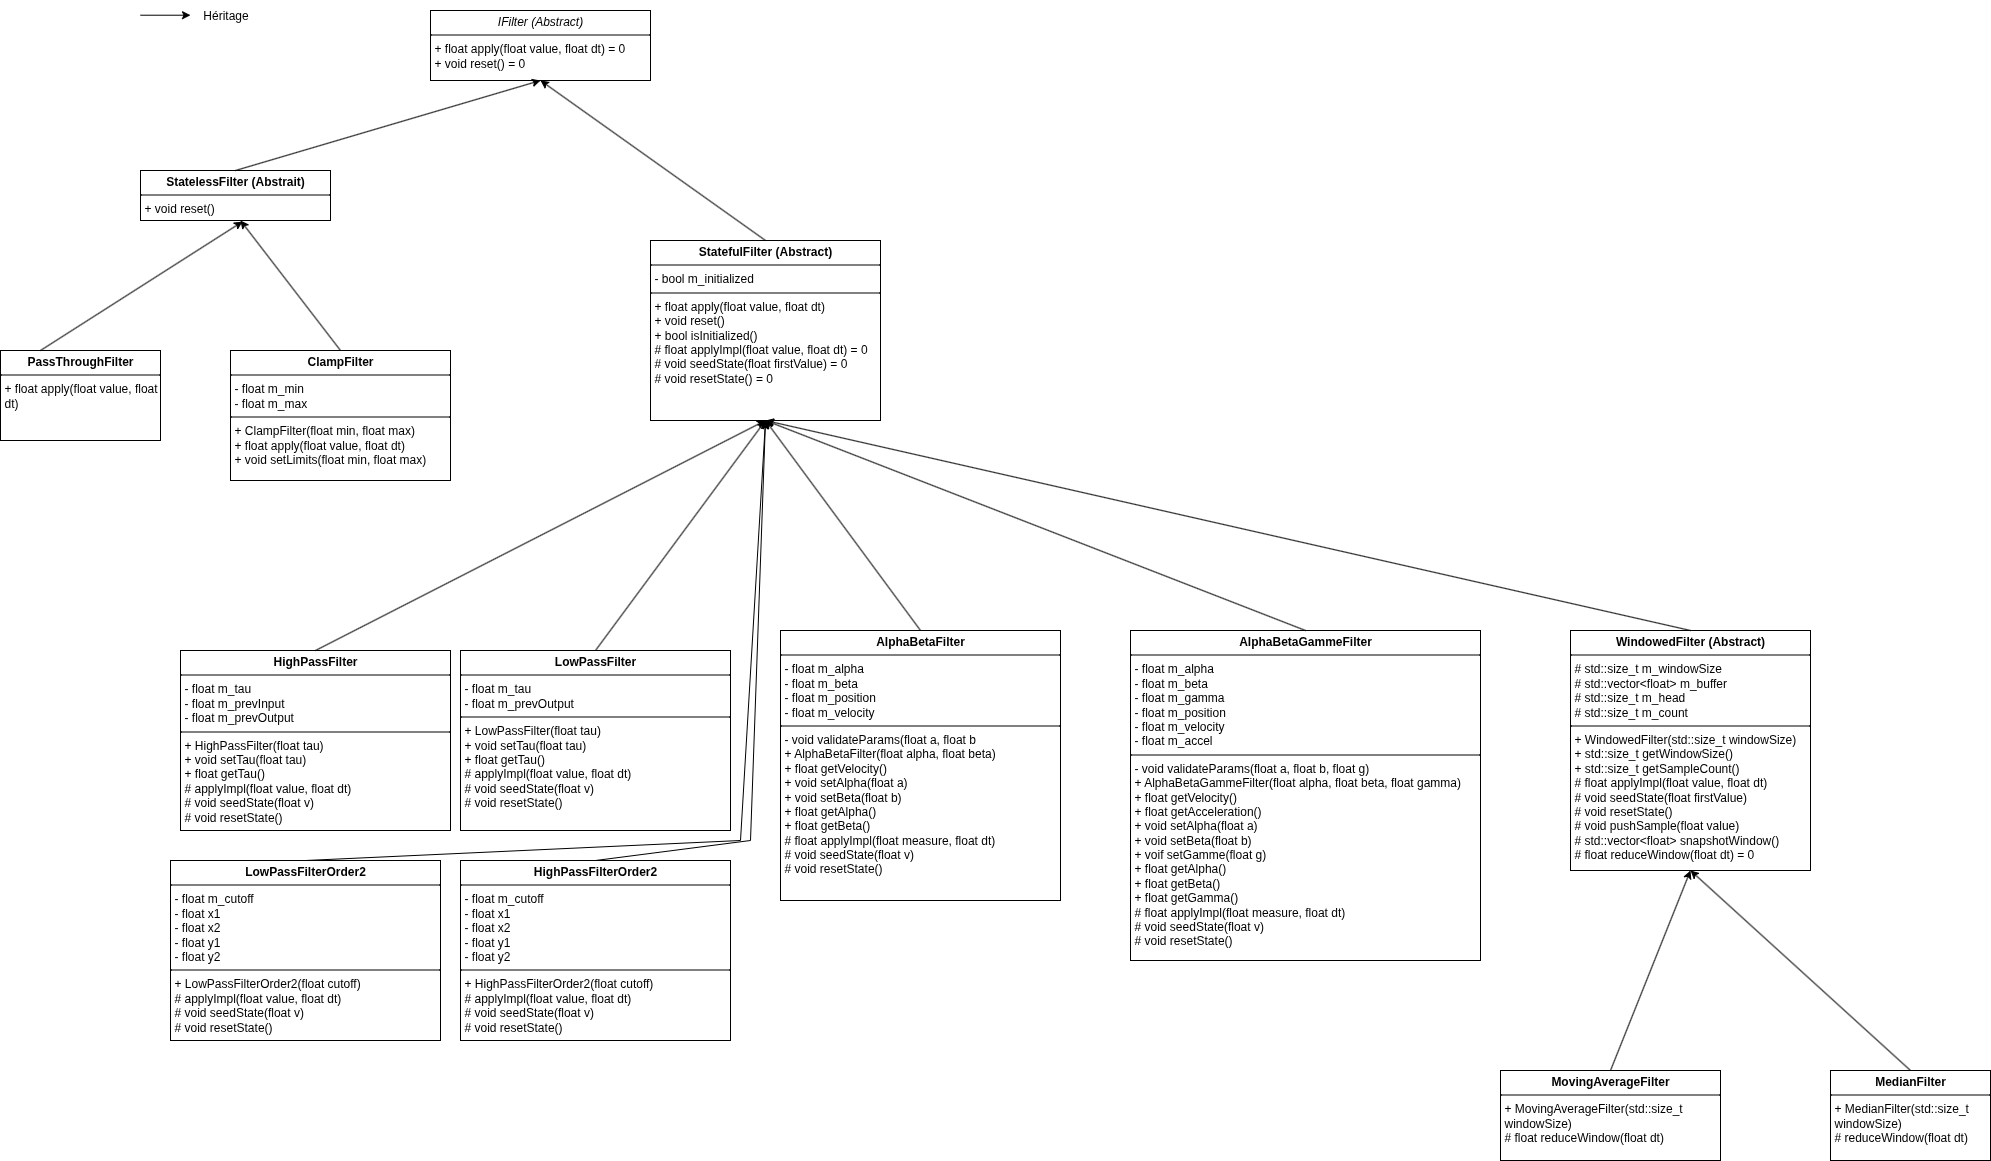
\includegraphics[width=\textheight]{images/diagramme_classe_filtre.png}
    \caption{Diagramme de classes des filtres}
    \label{fig:diagramme_classe_filtre}
\end{sidewaysfigure}


Pour faciliter l'implémentation de différents types de filtres, nous avons créé une classe abstraite 
\texttt{IFilter} qui définit une interface commune pour tous les filtres. Cette classe contient deux méthodes 
abstraites :
\begin{itemize}
    \item \texttt{float apply(float value, float dt)} : cette méthode prend en entrée une valeur à filtrer et un 
    intervalle de temps (dt) et retourne la valeur filtrée.
    \item \texttt{void reset()} : cette méthode réinitialise l'état interne du filtre, ce qui est utile pour les 
    filtres qui maintiennent un historique des valeurs précédentes
\end{itemize}

Nous avons aussi la classe abstraite \texttt{StatufulFilter} qui hérite de \texttt{IFilter} et qui est destinée 
aux filtres qui nécessitent de conserver un état interne, comme le filtre passe-bas et passe-haut. 
Cette classe contient des méthodes pour gérer l'état interne du filtre telles que l'initialisation, la mise à jour 
et la réinitialisation de l'état. \\

Il y a aussi la classe abstraite \texttt{WindowedFilter} qui hérite de \texttt{StatufulFilter} et qui est destinée 
aux filtres qui utilisent une fenêtre glissante pour traiter les données, comme le filtre médian. 
Cette classe contient des méthodes pour gérer la fenêtre glissante, telles que l'ajout de nouvelles valeurs, le
calcul sur la fenêtre et la réinitialisation de la fenêtre. \\

Nous allons nous pencher plus en détail sur les filtres passe-bas et médian, qui sont les deux types de filtres que nous avons décidé d'analyser 
parmi les différents types de filtres existants.

\subsubsection{Le filtre passe-Bas (ordre 1)}
\label{sec:filtre_passe_bas}

Le filtre passe-bas est le filtre le plus utilisé en automatique. Son objectif est d'atténuer les composantes de haute fréquence du signal tout en conservant les variations lentes représentant généralement l'information utile.

Dans le domaine de Laplace, la fonction de transfert d'un filtre passe-bas du premier ordre est donnée par :
\begin{equation}
    H(s) = \frac{1}{\tau s + 1}
\end{equation}

où : 
\begin{itemize}
    \item $\tau$ représente la constante de temps du filtre
    \item $s$ est la variable complexe de Laplace
\end{itemize}

A partir de cette fonction de transfert, il est possible de retrouver l'équation différentielle décrivant le comportement du filtre :
\begin{equation}
    \tau \frac{dy(t)}{dt} + y(t) = x(t)
\end{equation}

avec :
\begin{itemize}
    \item $x(t)$ le signal d'entrée
    \item $y(t)$ le signal filtré
\end{itemize}

Cette équation montre que la sortie ne suit pas instantanément l'entrée. Le filtre agit comme une moyenne glissante : lorsque l'entrée varie brutalement, la sortie évolue progressivement vers cette nouvelle valeur. \\

Comme le système développé fonctionne de manière discrète, cette équation est discrétisée en utilisant la méthode d'Euler arrière, conduisant aux équations suivantes :
\begin{equation}
    \alpha = \frac{\tau}{\tau + dt}
\end{equation}
\begin{equation}
    y[n] = \alpha y[n-1] + (1 - \alpha)x[n]
\end{equation}

où : 
\begin{itemize}
    \item $y[n]$ est la sortie filtrée à l'instant $n$
    \item $x[n]$ est l'entrée à l'instant $n$
    \item $y[n-1]$ est la sortie filtrée à l'instant $n-1$
    \item $\alpha$ est le coefficient de filtrage, qui dépend de la constante de temps $\tau$ et de l'intervalle 
    de temps $dt$
    \item $dt$ est l'intervalle de temps entre deux échantillons
    \item $\tau$ est la constante de temps du filtre
\end{itemize}

Le coefficient $\alpha$ contrôle directement le comportement du filtre.
\begin{itemize}
    \item Si $\alpha$ est proche de 1, le filtre utilise principalement les anciennes valeurs. Le filtrage est 
    fort mais le retard augmente
    \item Si $\alpha$ est proche de 0, le filtre suit rapidement le signal d'entrée mais atténué moins efficacement 
    le bruit.
\end{itemize}

A chaque appel de la fonction \texttt{apply()}, une seule nouvelle mesure est nécessaire, ainsi que la sortie calculée à l'itération précédente. Le filtre possède donc une mémoire minimale, ce qui en fait un algorithme très léger en calcul.

\paragraph{Evaluation}

Pour l'évaluation des performances du filtre passe-bas, on utilisera deux signaux, celui désiré et le bruit. Les valeurs sont générées comme ceci :
\begin{equation}
    y = \sin(2 \pi f_{low} \Delta t) + \sin(2 \pi f_{noise} \Delta t)
\end{equation}

où :
\begin{itemize}
    \item $f_{low}$ est la fréquence du signal désiré, ici de 10
    \item $f_{noise}$ est la fréquence du bruit, ici 200
    \item $\Delta t$ est l'intervalle de temps entre deux échantillons, ici 0.001
\end{itemize}

Le $\tau$ sera égal à $\frac{1}{2 \pi f_c}$, avec $f_c$ la fréquence de coupure du filtre, ici 15. \\

Le signal temporel (cf. figure \ref{fig:low_pass1}) montre que le filtre passe-bas atténue efficacement 
les oscillations rapides présentes sur le signal brut. La composante basse fréquence est correctement 
conservée et devient nettement plus visible après filtrage. \\

On remarque cependant que le signal filtré présente encore quelques oscillations résiduelles autour de la composante utile. Ce comportement est directement lié à la pente d'atténuation du filtre. \\

Une pente de 20 dB/décade signifie que lorsque la fréquence est multipliée par 10 (par exemple de 20 Hz à 200 Hz ou de 100 Hz à 1000 Hz), le gain du filtre diminue de 20 dB. Autrement dit, les hautes fréquences sont progressivement atténuées, mais pas supprimées instantanément. \\

Cette pente constitue une propriété fondamentale des filtres du premier ordre. Elle résulte directement de leur fonction de transfert, qui ne possède qu'un seul pôle. Par conséquent, les fréquences situées juste après la fréquence de coupure restent encore partiellement présentes dans le signal, ce qui explique que le bruit observé ne disparaisse pas complètement après filtrage. \\

\RemarkBox
{Remarque}
{
Le filtrage introduit également un léger retard temporel entre le signal brut et le signal filtré, phénomène 
inhérent à tous les filtres causaux.
}

\RemarkBox{Origine de la pente d'atténuation}
{
Pour un filtre du premier ordre, le gain décroît approximativement comme $$|H(j\omega)|\propto\frac1{\omega}$$ aux hautes fréquences. En exprimant ce gain en décibels, $$G_{dB}=20\log_{10}|H(j\omega)|$$ on montre que chaque multiplication de la fréquence par dix entraîne une diminution du gain de 20 dB. C'est pourquoi un filtre du premier ordre possède une pente de -20 dB/décade.
}

L'analyse fréquentielle (cf. figure \ref{fig:low_pass_fft1}) confirme ce comportement. Le spectre brut est constitué de deux composantes principales :
\begin{itemize}
    \item une composante utile située à 10 Hz
    \item une composante parasite située à 200 Hz
\end{itemize}

Après filtrage :
\begin{itemize}
    \item la composante de 10 Hz est quasiment conservée
    \item la composante de 200 Hz est fortement atténuée mais reste visible
\end{itemize}

Le filtre réalise donc bien sa fonction de passe-bas mais ne supprime pas complètement les hautes fréquences. \\

La densité spectrale de puissance (PSD) (cf. figure \ref{fig:low_pass_psd1}) confirme aussi ces observations. La puissance associée aux hautes fréquences diminue fortement après filtrage. Toutefois, une partie de l'énergie demeure présente autour de 200 Hz. Cette observation est cohérente avec les propriétés théoriques du filtre passe-bas.

\begin{figure}
    \centering
    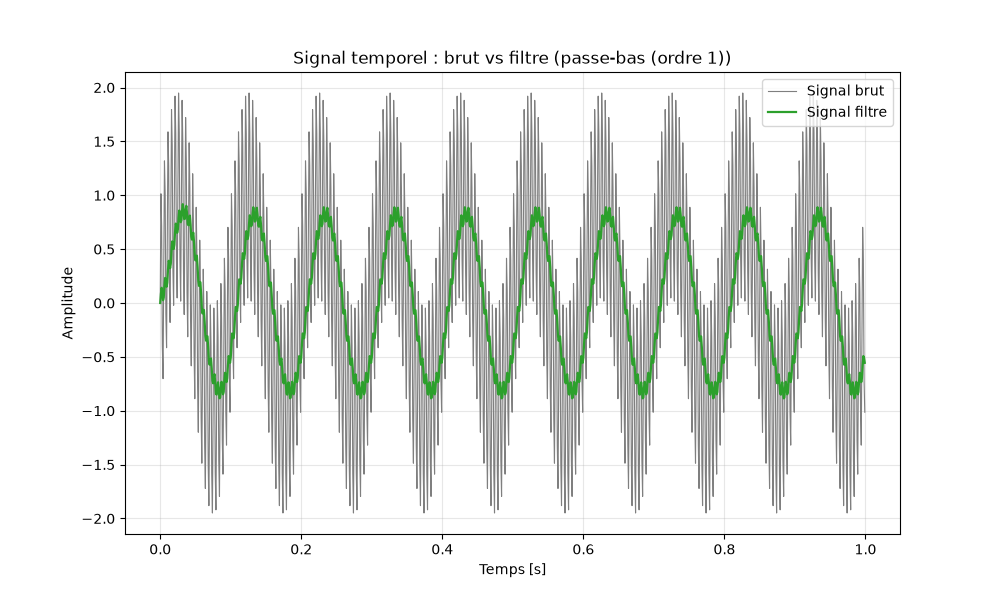
\includegraphics[width=\textwidth]{images/low_pass_order1.png}
    \caption{Résultat du filtre passe-bas d'ordre 1 sur des fréquences avec du bruit}
    \label{fig:low_pass1}
\end{figure}

\begin{figure}
    \centering
    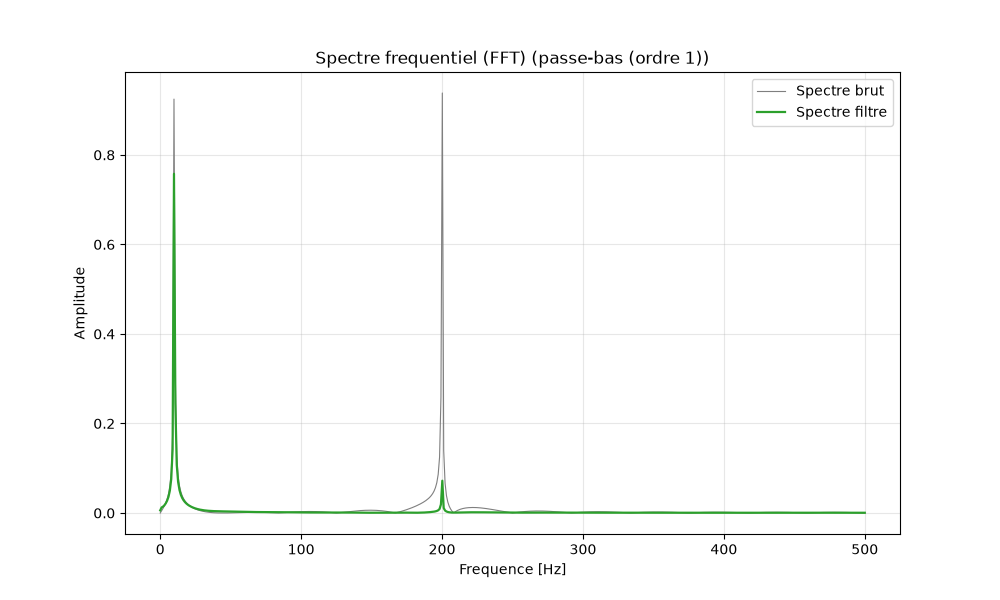
\includegraphics[width=\textwidth]{images/low_pass_fft_order1.png}
    \caption{Spectre fréquentiel du signal avant et après filtre passe-bas d'ordre 1}
    \label{fig:low_pass_fft1}
\end{figure}




\paragraph{Avantages}

\begin{itemize}
    \item Coût de calcul très faible
    \item Implémentation simple
    \item Parfaitement adapté aux systèmes embarqués
\end{itemize}

\paragraph{Inconvénients}

\begin{itemize}
    \item Retard introduit sur la mesure
    \item Pente d'atténuation limitée à 20 dB/décade
    \item Performances limitées lorsque le bruit possède une énergie importante proche de la fréquence de coupure
\end{itemize}

\subsubsection{Le filtre passe-Haut (ordre 1)}
\label{sec:filtre_passe_haut}

Le filtre passe-haut réalise l'opération inverse.

Son objectif est de supprimer les composants lents du signal, telles que les dérives ou les offsets des capteurs, afin de ne conserver que les variations rapides.

Sa fonction de transfert est :
\begin{equation}
    H(s) = \frac{\tau s}{1 + \tau s}
\end{equation}

Cette fonction conduit à l'équation :
\begin{equation}
    \tau \frac{dy(t)}{dt} + y(t) = \tau \frac{dx(t)}{dt}
\end{equation}

Le filtre réagit donc essentiellement aux variations du signal. Après discrétisation, on obtient :
\begin{equation}
    \alpha = \frac{\tau}{\tau + \Delta t}
\end{equation}
\begin{equation}
    y[n] = \alpha (y[n-1] + x[n] - x[n-1])
\end{equation}

où :
\begin{itemize}
    \item $y[n]$ est la sortie filtrée à l'instant $n$
    \item $x[n]$ est l'entrée à l'instant $n$
    \item $y[n-1]$ est la sortie filtrée à l'instant $n-1$
    \item $x[n-1]$ est l'entrée à l'instant $n-1$
    \item $\Delta t$ est l'intervalle de temps entre deux échantillons
    \item $\tau$ est la constante de temps du filtre
    \item $\alpha$ est le coefficient de filtrage, qui dépend de la constante de temps $\tau$ et de l'intervalle 
    de temps $\Delta t$
\end{itemize}

Le filtre mémorise simultanément la dernière valeur d'entrée et la dernière valeur de sortie, ce qui lui permet de réagir aux variations du signal. \\

\paragraph{Evaluation}

Pour l'évaluation des performances du filtre passe-haut, on va prendre deux signaux, celui désiré et le bruit. les valeurs sont générées comme ceci :
\begin{equation}
    y = \sin(2 \pi f_{noise} \Delta t) + \sin(2 \pi f_{high} \Delta t)
\end{equation}

où : 
\begin{itemize}
    \item $f_{high}$ est la fréquence du signal désiré, ici de 100
    \item $f_{noise}$ est la fréquence du bruit, ici 10
    \item $\Delta t$ est l'intervalle de temps entre deux échantillons, ici 0.001
\end{itemize}

Le $\tau$ sera égal à $\frac{1}{2 \pi f_c}$, avec $f_c$ la fréquence de coupure du filtre, ici 80. \\

Le filtre passe-haut élimine efficacement une grande partie des composantes de basse fréquence présentes dans le signal. Après filtrage, seule la sinusoïde de haute fréquence reste visible (cf. figure \ref{fig:high_pass1}). \\

L'analyse fréquentielle (cf. figure \ref{fig:high_pass_fft1}) confirme ce comportement. Le spectre brut est constitué de deux composantes principales :
\begin{itemize}
    \item une composante parasite située à 10 Hz
    \item une composante utile située à 100 Hz
\end{itemize}

Après filtrage :
\begin{itemize}
    \item la composante de 10 Hz est fortement réduite
    \item la composante de 100 Hz est quasiment conservée
\end{itemize}

Toutefois, un fiable résidu subsiste à basse fréquence. \\

La densité spectrale de puissance (cf. figure \ref{fig:high_pass_psd1}) confirme aussi ces observations. La puissance des basses fréquences diminue fortement après filtrage. Toutefois, une partie de l'énergie demeure présente autour de 10 Hz. Cette observation est cohérente avec les propriétés théoriques du filtre passe-haut.

\begin{figure}
    \centering
    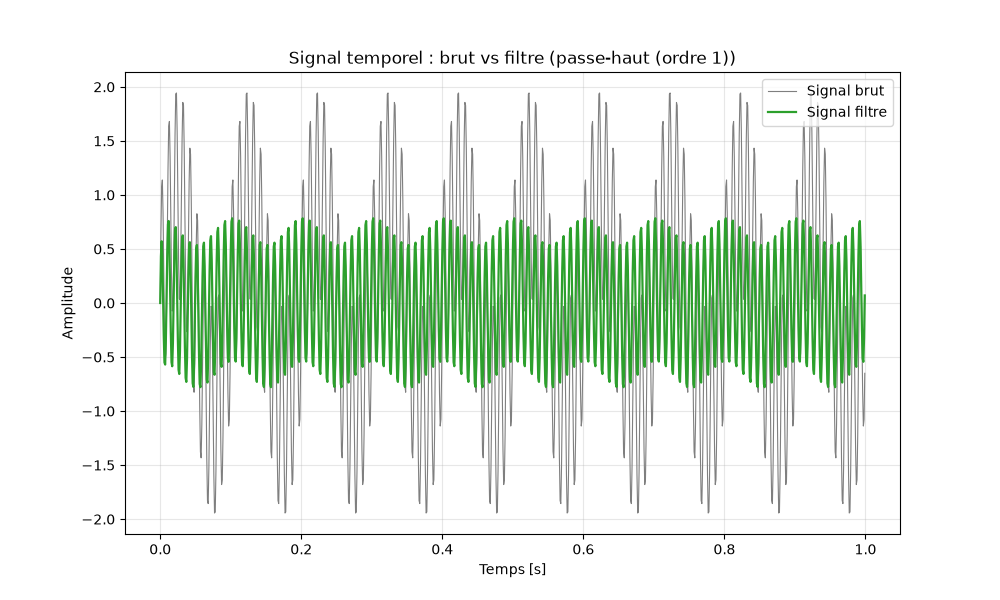
\includegraphics[width=\textwidth]{images/high_pass_order1.png}
    \caption{Résultat du filtre passe-haut d'ordre 1 sur des fréquences avec du bruit}
    \label{fig:high_pass1}
\end{figure}

\begin{figure}
    \centering
    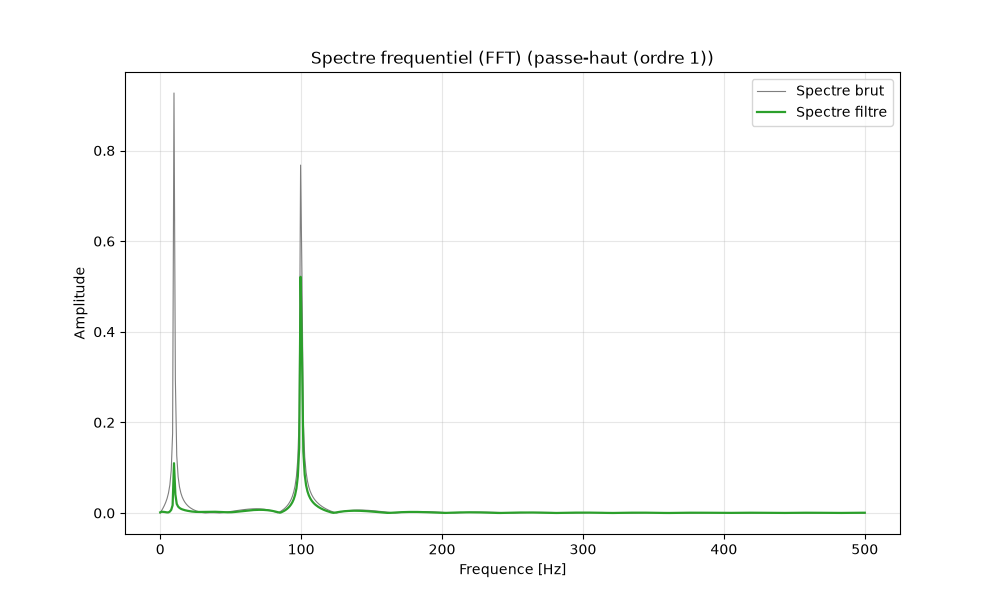
\includegraphics[width=\textwidth]{images/high_pass_fft_order1.png}
    \caption{Spectre fréquentiel du signal avant et après filtre passe-haut d'ordre 1}
    \label{fig:high_pass_fft1}
\end{figure}



\paragraph{Avantages}

\begin{itemize}
    \item Suppression des offsets
    \item Elimition des dérives lentes
\end{itemize}

\paragraph{Inconvénients}

\begin{itemize}
    \item Amplification du bruit haute fréquence
    \item Rarement utilisé seul pour filtrer une mesure.
\end{itemize}

\subsubsection{Le filtre Butterworth (ordre 2)}
\label{sec:filtre_butterworth}

Comme expliqué précédemment, un filtre du premier ordre possède une pente asymptotique de -20 dB/décade, ce qui signifie que son atténuation augmente relativement lentement lorsque la fréquence dépasse la fréquence de coupure. Les composantes fréquentielles proches de cette fréquence restent donc encore partiellement présentes dans le signal. Pour améliorer les performances du filtrage, il est nécessaire d'augmenter l'ordre du filtre. \\

Un filtre d'ordre 2 possède deux pôles. Chaque pôle apportant une pente supplémentaire de 20 dB/décade, un filtre du second ordre atteint une pente de -40 dB/décade, ce qui permet une atténuation beaucoup plus rapide des hautes fréquences. Parmi les différentes familles existantes, les filtres Butterworth constituent un excellent compromis entre simplicité, stabilité et qualité de filtrage. \\

Le filtre de Butterworth a été proposé par Stephen Butterworth en 1930 afin d'obtenir une réponse fréquentielle maximalement plate dans la bande passante. Cette propriété signifie que le gain reste pratiquement constant jusqu'à la fréquence de coupure, sans oscillation ni ondulation, ce qui permet de préserver les informations utiles du signal tout en améliorant fortement l'atténuation des hautes fréquences. \\

Un filtre de Butterworth d'ordre 2 a été développé pour remplacer le filtre passe-bas du premier ordre et passe-haut du premier ordre. \\

Sa fonction de transfert est :
\begin{equation}
    H(s) = \frac{\omega^{2}_{c}}{s^{2} + \sqrt{2}\omega_{c}s + \omega^{2}_{c}}
\end{equation}
\begin{equation}
    w_{c} = 2\pi f_{c}
\end{equation}

Contrairement aux filtres précédents, cette fonction possède deux pôles. Le filtre dépend donc non seulement de la mesure actuelle mais également des deux mesures précédentes ainsi que des deux sorties précédentes. \\

Après discrétisation, l'équation générale devient :

\begin{equation}
    y[n] = b_{0}x[n] + b_{1}x[n-1] + b_{2}x[n-2] - a_{1}y[n-1] - a_{2}y[n-2]
\end{equation}

Les coefficients $a_{i}$ et $b_{i}$ sont recalculés à partir de la fréquence de coupure, de l'intervalle de temps entre deux mesures et du facteur de qualité $Q = \frac{1}{\sqrt{2}}$ qui correspond précisément au filtre de Butterworth. \\

Contrairement au filtre du premier ordre, le filtre utilise quatre états internes, qui sont les deux anciennes entrées et deux anciennes sorties. Cette mémoire supplémentaire lui permet d'obtenir une pente d'atténuation de 40 dB/décade, soit deux fois plus importante que celle du filtre du premier ordre. \\

Ce qui change entre le filtre passe-haut et passe-bas d'ordre 2, ce sont les coefficients $a_{i}$ et $b_{i}$ qui sont recalculés en fonction de la fréquence de coupure et du type de filtre. \\

Pour le filtre passe-bas :
\begin{equation}
    \begin{cases}
        a_{0} = 1 + \alpha \\
        a_{1} = \frac{-2 * \cos(\omega)}{a_{0}} \\
        a_{2} = \frac{1 - \alpha}{a_{0}} \\
        b_{0} = \frac{\frac{1 - \cos(\omega)}{2}}{a_{0}} \\
        b_{1} = \frac{1 - \cos(\omega)}{a_{0}} \\
        b_{2} = \frac{\frac{1 - \cos(\omega)}{2}}{a_{0}} \\
    \end{cases}
\end{equation}

Pour le filtre passe-haut :
\begin{equation}
    \begin{cases}
        a_{0} = 1 + \alpha \\
        a_{1} = \frac{-2 * \cos(\omega)}{a_{0}} \\
        a_{2} = \frac{1 - \alpha}{a_{0}} \\
        b_{0} = \frac{(1 + \cos(\omega)) * 0.5}{a_{0}} \\
        b_{1} = \frac{-(1 + \cos(\omega))}{a_{0}} \\
        b_{2} = \frac{(1 + \cos(\omega)) * 0.5}{a_{0}} \\
    \end{cases}
\end{equation}

où :
\begin{equation}
    \alpha = \frac{\sin(\omega)}{2 * Q}
    \omega = \frac{2 \pi * f_c}{fs}
    fs = \frac{1}{\Delta t} 
\end{equation}

\RemarkBox
{Remarque}
{
    Pour les évaluations, nous avons choisi de conserver les mêmes signaux que pour les filtres du premier ordre 
    ainsi que des mêmes fréquences de coupure. Cela permet de comparer directement les performances des filtres 
    d'ordre 1 et d'ordre 2.
}

\paragraph{Evaluation du filtre passe-bas Butterworth d'ordre 2}

Le signal filtré obtenu avec le filtre de Butterworth apparaît beaucoup plus lisse. Les oscillations rapides ont pratiquement disparu et la sinusoïde basse fréquence est conservée avec une très bonne fidélité (cf. figure \ref{fig:low_pass2}). Par rapport au filtre d'ordre 1, la composante utile est plus propre et présente moins de fluctuations parasites. On observe néanmoins un retard légèrement supérieur, conséquence directe de l'augmentation de l'ordre du filtre. \\

Le spectre fréquentiel met clairement en évidence les performances du filtre (cf. figure \ref{fig:low_pass_fft1}) où la composante utile de 10 Hz est quasiment inchangée. En revanche, la composante de 200 Hz est presque entièrement supprimée. Cette différence est directement liée à la pente d'atténuation de 40 dB/décade du filtre de Butterworth. \\

La densité spectrale de puissance (cf. figure \ref{fig:low_pass_psd2}) confirme l'amélioration, la puissance du bruit haute fréquence est nettement plus faible que pour le filtre d'ordre 1. Au-delà de 250 Hz, l'énergie résiduelle ne devient pratiquement nulle. Le filtre élimine donc beaucoup plus efficacement les hautes fréquences. \\

\begin{figure}
    \centering
    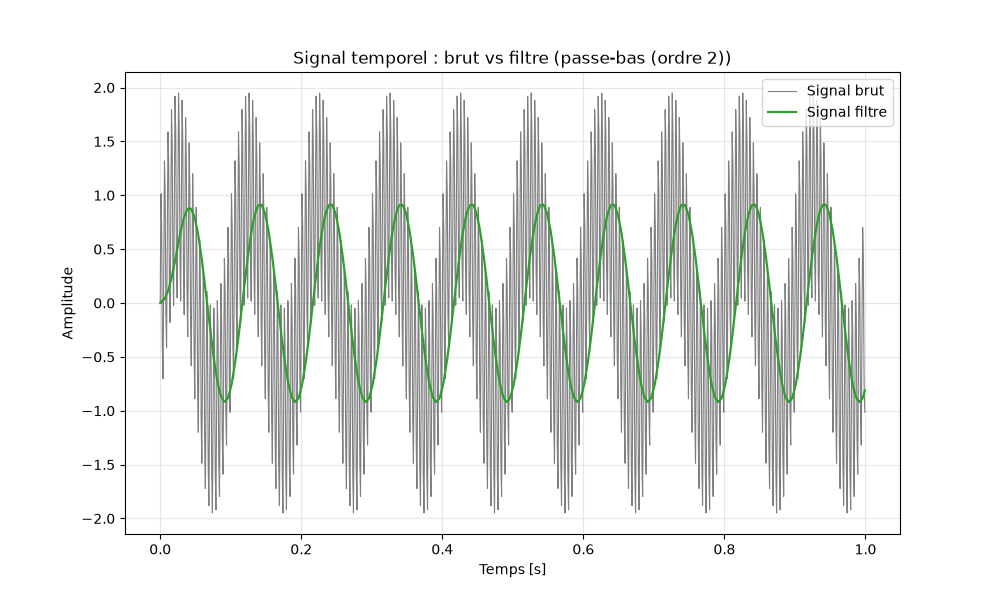
\includegraphics[width=\textwidth]{images/low_pass_order2.png}
    \caption{Résultat du filtre passe-bas d'ordre 2 sur des fréquences avec du bruit}
    \label{fig:low_pass2}
\end{figure}

\begin{figure}
    \centering
    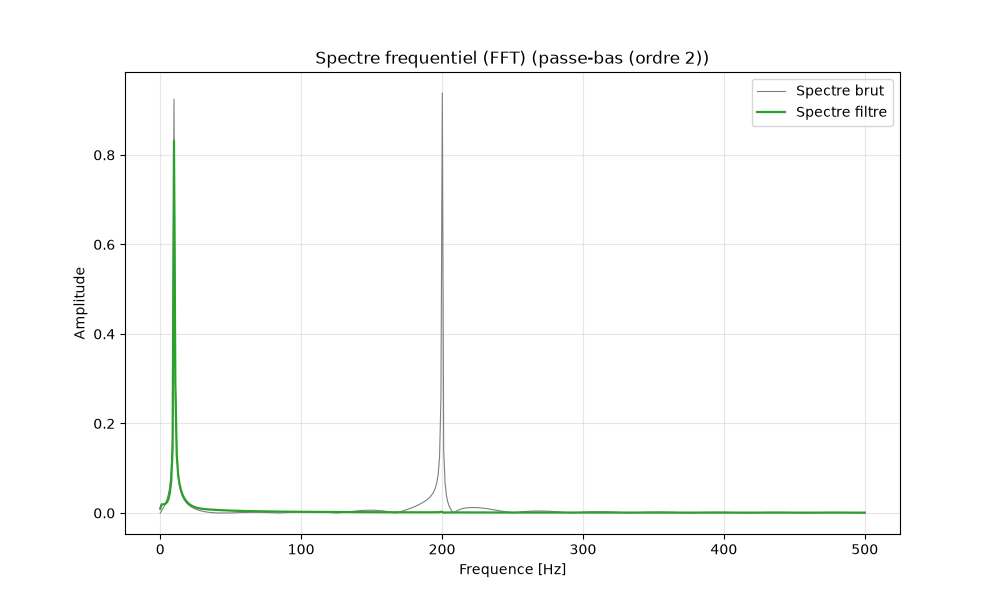
\includegraphics[width=\textwidth]{images/low_pass_fft_order2.png}
    \caption{Spectre fréquentiel du signal avant et après filtre passe-bas d'ordre 2}
    \label{fig:low_pass_fft2}
\end{figure}



\paragraph{Evaluation du filtre passe-haut Butterworth d'ordre 2}

Le signal filtré obtenu avec le filtre passe-haut de Butterworth d'ordre 2 est beaucoup plus régulier que celui obtenu avec le filtre d'ordre 1 (cf. figure \ref{fig:high_pass2}). La composante basse fréquence est pratiquement absente, la sinusoïde haute fréquence est conservée avec une amplitude presque constante. Contrairement au filtre d'ordre 1, on ne distringue pratiquement plus de modulation d'amplitude. Cela traduit une meilleure suppression des basses fréquences. \\

Le spectre fréquentiel (cf. figure \ref{fig:high_pass_fft2}) montre une différence particulièrement nette entre les deux filtres. La composante de 10 Hz disparaît presque complètement, tandis que la composante de 100 Hz est parfaitement conservée. Le filtre réalise donc une séparation fréquentielle beaucoup plus efficace. \\

La densité spectrale de puissance (cf. figure \ref{fig:high_pass_psd2}) montre une diminution très importante de la puissance des basses fréquences. La composante utile est conservée alors que les fréquences indésirables sont fortement atténuées. \\

\begin{figure}
    \centering
    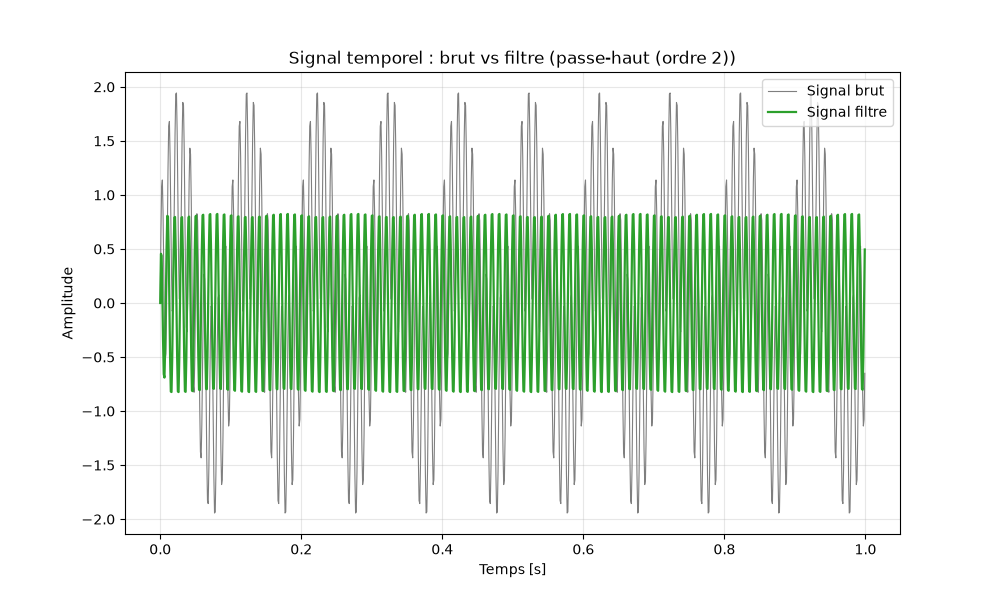
\includegraphics[width=\textwidth]{images/high_pass_order2.png}
    \caption{Résultat du filtre passe-haut d'ordre 2 sur des fréquences avec du bruit}
    \label{fig:high_pass2}
\end{figure}

\begin{figure}
    \centering
    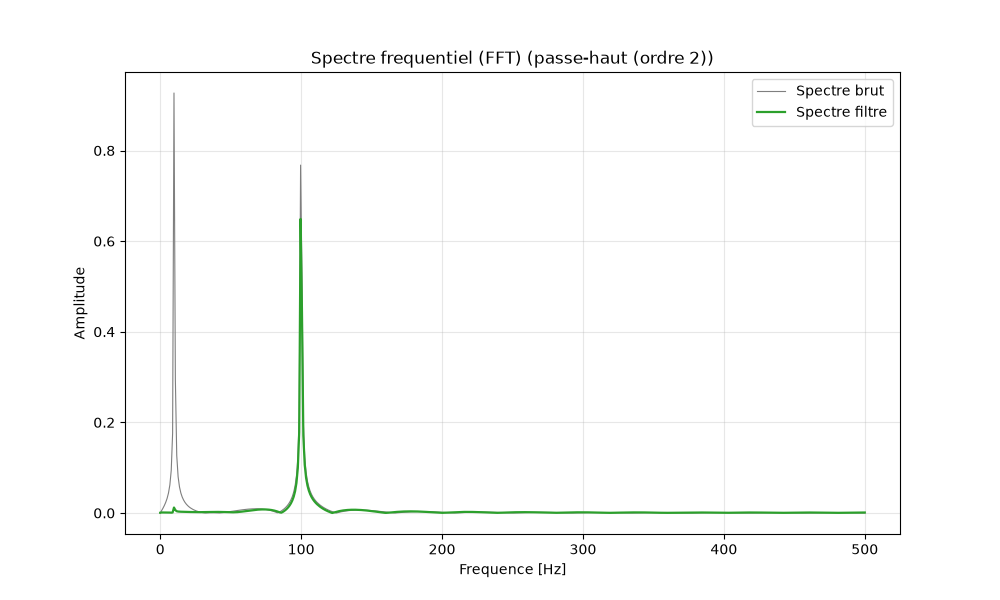
\includegraphics[width=\textwidth]{images/high_pass_fft_order2.png}
    \caption{Spectre fréquentiel du signal avant et après filtre passe-haut d'ordre 2}
    \label{fig:high_pass_fft2}
\end{figure}



\paragraph{Conclusion}

Le filtre Butterworth peut être considéré comme une évolution naturelle des filtres du premier ordre. Il conserve les mêmes objectifs de filtrage, il préserve beaucoup mieux les fréquences désirées tout en atténuant plus efficacement les fréquences indésirables. Ils ont une excellente stabilité numérique, mais cela a un coût de calcul plus élevé que le filtre du premier ordre.

\subsubsection{Le filtre médian}
\label{sec:filtre_median}

\paragraph{Principe}

Le filtre médian est un filtre non-linéaire qui remplace chaque valeur d'un signal par la médiane des valeurs voisines dans une fenêtre glissante. Contrairement aux filtres linéaires, le filtre médian est particulièrement efficace pour éliminer les pics de bruit tout en préservant les bords et les détails du signal. \\

\paragraph{Fonctionnement}

Le filtre médian est de type WindowedFilter, ce qui signifie qu'il utilise une fenêtre glissante pour traiter les données. La taille de cette fenêtre est un paramètre clé du filtre, car elle détermine le nombre de valeurs voisines à considérer pour calculer la médiane. Il fonctionne en 3 étapes :
\begin{enumerate}
    \item Pour chaque point, il ajoute sa valeur dans un tableau de taille fixe (la taille de la fenêtre)
    \item Il récupère les valeurs du tableau et les trie par ordre croissant
    \item Il retourne la valeur médiane du tableau trié
\end{enumerate}

\paragraph{Exemple d'utilisation}

Dans notre exemple, nous avons utilisé un signal sinusoïdal avec des pics de bruit aléatoires pour illustrer l'effet du filtre médian sur le signal. Le signal est défini par l'équation suivante : 

$$y = \sin(2 * \pi * 0.2 * t) + spike$$

Où : 
\begin{itemize}
    \item $y$ est la valeur du signal à l'instant $t$
    \item $t$ est le temps en secondes
    \item $spike$ est un pic de bruit aléatoire qui est égal à 2 toutes les 2 secondes et à 0 sinon
\end{itemize}

On a appliqué le filtre médian sur ce signal avec une fenêtre de taille 5 et on a obtenu le résultat présenté dans la figure \ref{fig:median}. On peut voir que le filtre médian a réussi à éliminer les pics de bruit tout en préservant la forme générale du signal sinusoïdal. \\

\begin{figure}
    \centering
    
\includegraphics[width=\textwidth]{images/median.png}
    \caption{Résultat du filtre médian sur des fréquences avec des pics de bruit, avec une fenêtre de 5}
    \label{fig:median}
\end{figure}

\paragraph{Avantages et Inconvénients}

Le filtre médian présente plusieurs avantages par rapport aux filtres linéaires, notamment sa capacité à éliminer efficacement les pics de bruit tout en préservant les bords et les détails du signal. Cependant, il a également quelques inconvénients, tels qu'en fonction de la taille de la fenêtre, il peut introduire un décalage temporel dans le signal filtré et peut rendre un signal qui était continu en un signal discontinu (cf. figures \ref{fig:median_10} et \ref{fig:median_15}) \\

\begin{figure}
    \centering
    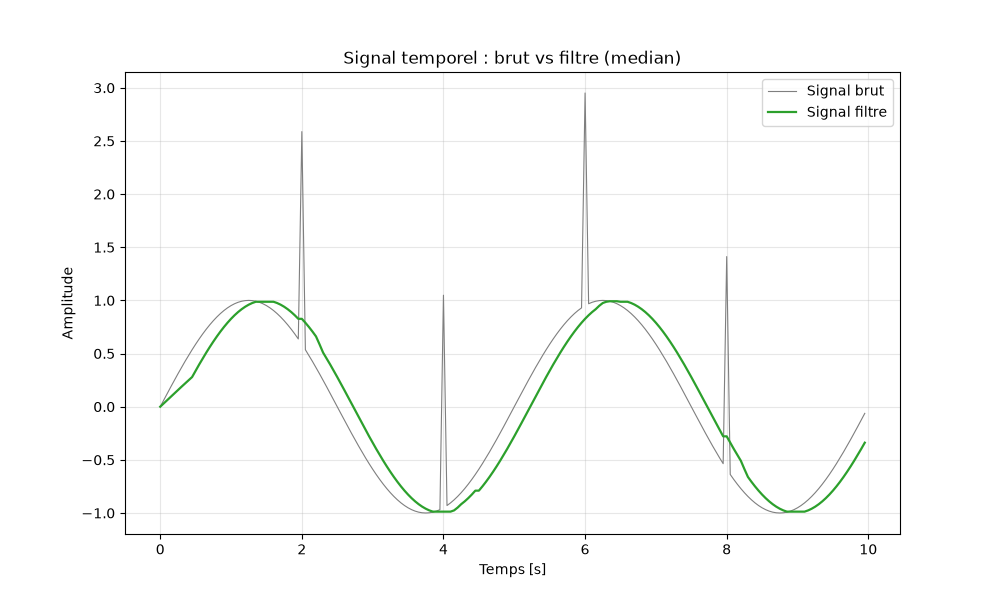
\includegraphics[width=\textwidth]{images/median_10.png}
    \caption{Résultat du filtre médian sur des fréquences avec des pics de bruit, avec une fenêtre de 10}
    \label{fig:median_10}
\end{figure}

\begin{figure}
    \centering
    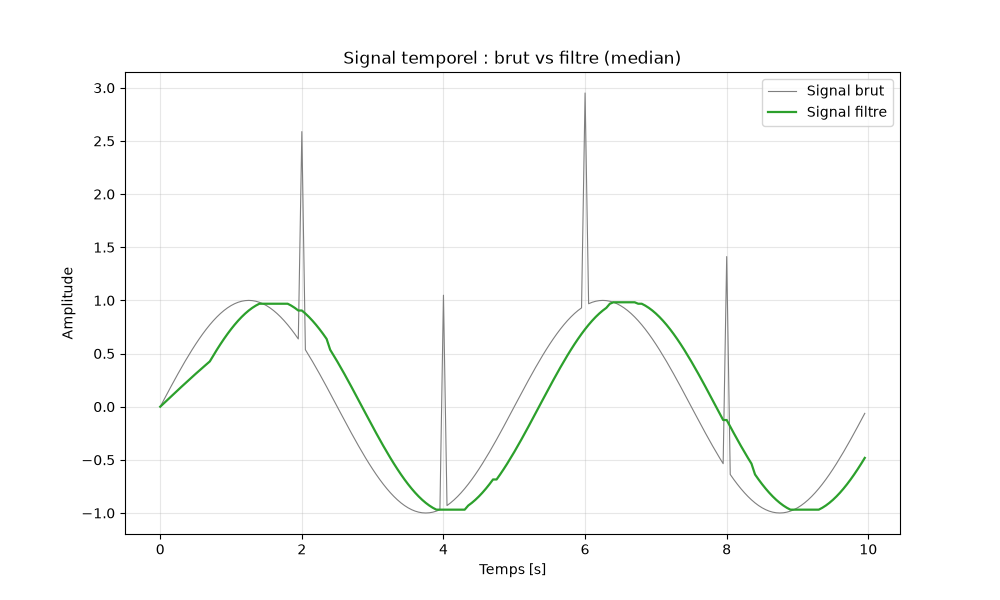
\includegraphics[width=\textwidth]{images/median_15.png}
    \caption{Résultat du filtre médian sur des fréquences avec des pics de bruit, avec une fenêtre de 15}
    \label{fig:median_15}
\end{figure}

\subsubsection{Evaluation des filtres sur des signaux d'instruments de musique}
\label{sec:instruments}

Nous allons maintenant utiliser nos filtres passe-bas et passe-haut d'ordre 2 pour filtrer des signaux réalistes provenant d'instruments de musique. Pour notre exemple, nous avons choisi un projet musical issu de la plateforme \href{https://cambridge-mt.com/}{Cambridge Music Technology} se prénommant "Timeless (Part 2)" de l'artiste MekaPhil. Nous avons extrait les pistes audio de la basse, de la guitare électrique et de la flûte, pour avoir une piste audio mixée contenant les trois instruments\footnote{Cette piste audio dure 4 secondes au lieu de 30 secondes pour faciliter les coûts de calcul}. \\


L'objectif de cette expérimentation est de vérifier si un filtre passe-bande, obtenu par la combinaison d'un filtre passe-bas et un filtre passe-haut, permet d'isoler la bande fréquentielle caractéristique d'un instrument présent dans un signal audio composé de plusieurs instruments. Pour chaque instrument, trois signaux sont comparés :
\begin{itemize}
    \item la piste originale de l'instrument (référence)
    \item le signal audio contenant le mélange des instruments
    \item le signal obtenu après filtrage du mélange.
\end{itemize}

L'analyse repose alors sur la transformée de Fourier (FFT) et la densité spectrale de puissance (PSD). \\

Pour chaque instrument, nous avons choisi des fréquences de coupure pour le filtre passe-bas et le filtre passe-haut afin de ne conserver que les fréquences de l'instrument. Les fréquences de coupure ont été choisies en fonction des caractéristiques fréquentielles de chaque instrument et qui sont les suivantes :
\begin{itemize}
    \item Basse : 30 Hz à 250 Hz
    \item Guitare électrique : 280 Hz à 900 Hz
    \item Flûte : 1000 Hz à 1400 Hz
\end{itemize}

\RemarkBox
{Remarque}
{
Ces fréquences ont été choisies via un \href{https://www.studioenregistrement.fr/post/frequences-des-instruments-de-musique}{tableau des fréquences des instruments de musique} mais aussi via l'analyse fréquentielle de chaque piste audio des instruments seules (cf. figures \ref{fig:bass_fft}, \ref{fig:guitar_fft} et \ref{fig:flute_fft}). 
}

\paragraph{Analyse des résultats de la basse}

La FFT de la basse seule (cf. figure \ref{fig:bass_fft}) montre que son énergie est principalement concentrée sous 250 Hz, ce qui est conforme à la littérature concernant les fréquences fondamentales de la basse. Après filtrage du mélange entre 30 Hz et 250 Hz, on observe que :
\begin{itemize}
    \item les composantes situées dans cette bande sont correctement conservées
    \item les composantes de moyenne et haute fréquence sont fortement atténuées
\end{itemize}

En revanche, la FFT du signal filtré montre encore quelques composantes résiduelles provenant d'autres instruments. Cette observation est normale puisque certains instruments produisent également des harmoniques dans les basses fréquences. \\

La densité spectrale de puissance (cf. figure \ref{fig:bass_psd}) confirme ce résultat. La puissance du signal filtré est concentrée dans la bande étudiée, tandis que les fréquences supérieures présentent une forte diminution de puissance. La décroissance importante observée après 250 Hz traduit le bon fonctionnement du passe-bas. \\

Le filtre permet de mettre en évidence les fréquences caractéristiques de la basse mais ne supprime pas totalement les autres instruments. \\

\begin{figure}
    \centering
    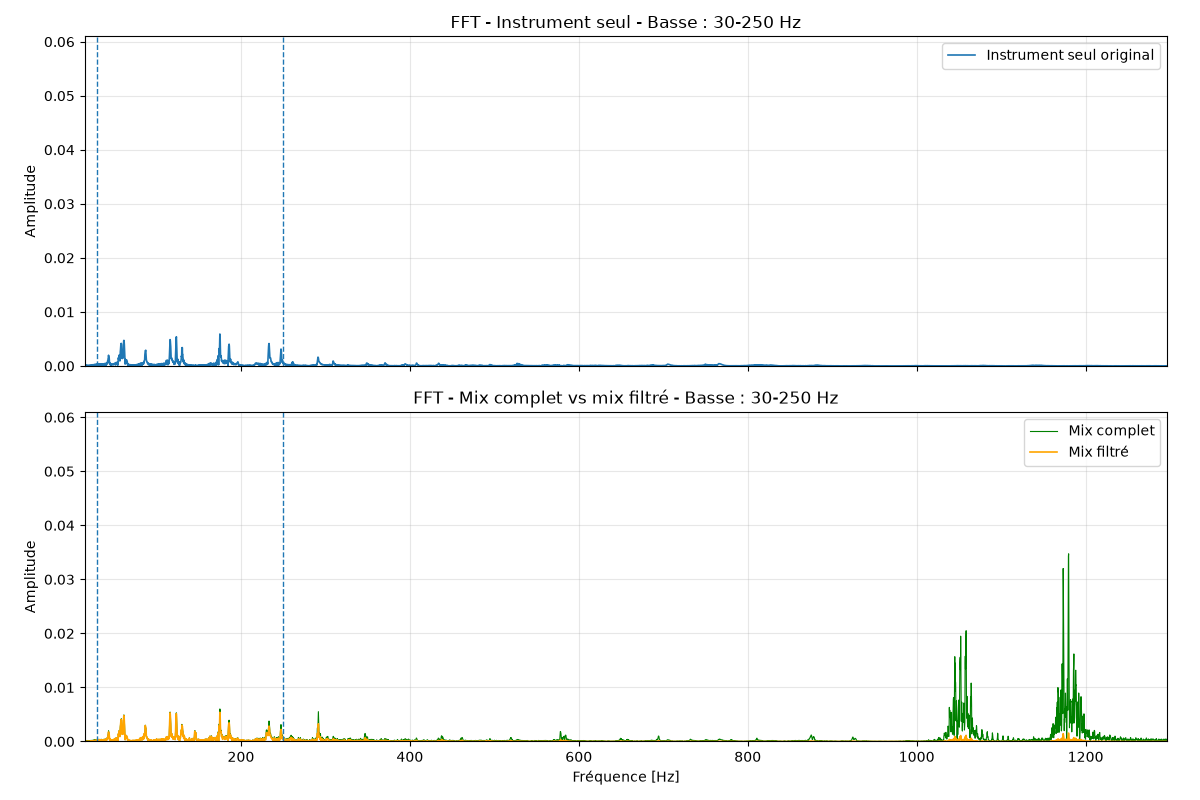
\includegraphics[width=\textwidth]{images/bass_fft.png}
    \caption{Spectre fréquentiel de la piste audio de la basse}
    \label{fig:bass_fft}
\end{figure}

\begin{figure}
    \centering
    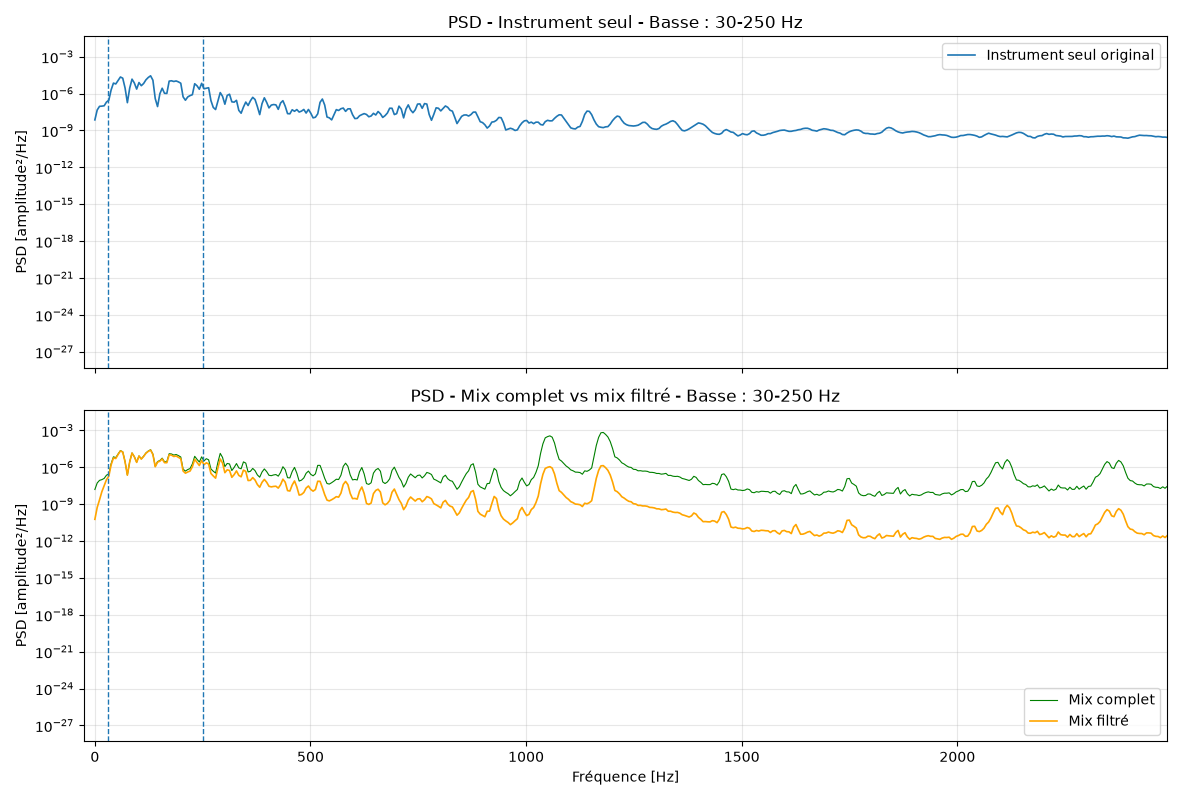
\includegraphics[width=\textwidth]{images/bass_psd.png}
    \caption{Densité spectrale de puissance de la piste audio de la basse}
    \label{fig:bass_psd}
\end{figure}

\paragraph{Analyse des résultats de la guitare électrique}

La FFT de la guitare électrique seule (cf. figure \ref{fig:guitar_fft}) montre une énergie répartie sur une plage relativement large. Le signal filtré conserve correctement les pics principaux présents dans cette bande. Cependant plusieurs composantes situées au-dessus de 1000 Hz subsistent dans le mélange. Cela s'explique par les nombreuses harmoniques produites par la guitare, mais également par les autres instruments. Le filtre réduit leur influence sans pouvoir les supprimer complètement. \\

La densité spectrale de puissance (cf. figure \ref{fig:guitar_psd}) montre une forte réduction de puissance en dehors de la bande sélectionnée. En revanche, la puissance dans la bande 280-900 Hz reste très proche de celle observée sur le signal original. Cette observation confirme que le filtre conserve efficacement la partie utile du signal. \\

La guitare est correctement mise en évidence. Les composantes principales sont conservées alors que les autres fréquences sont largement atténuées. \\

\begin{figure}
    \centering
    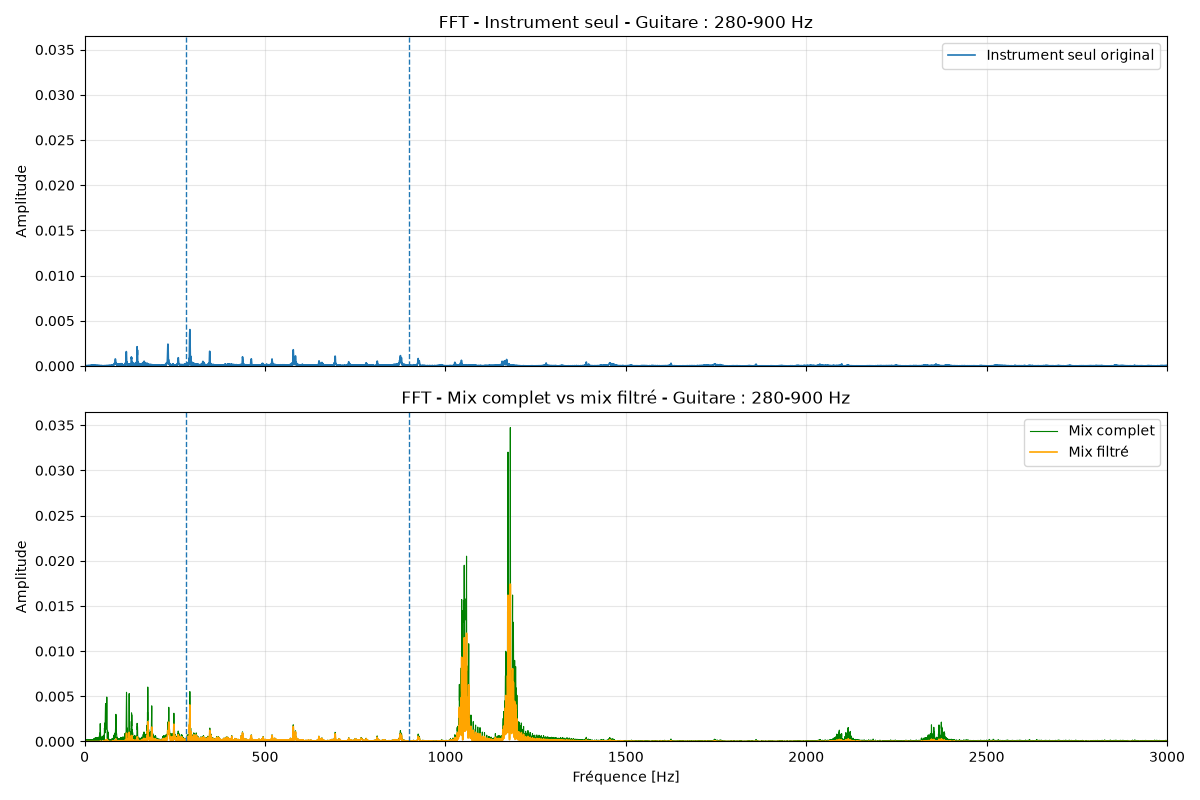
\includegraphics[width=\textwidth]{images/guitar_fft.png}
    \caption{Spectre fréquentiel de la piste audio de la guitare}
    \label{fig:guitar_fft}
\end{figure}

\begin{figure}
    \centering
    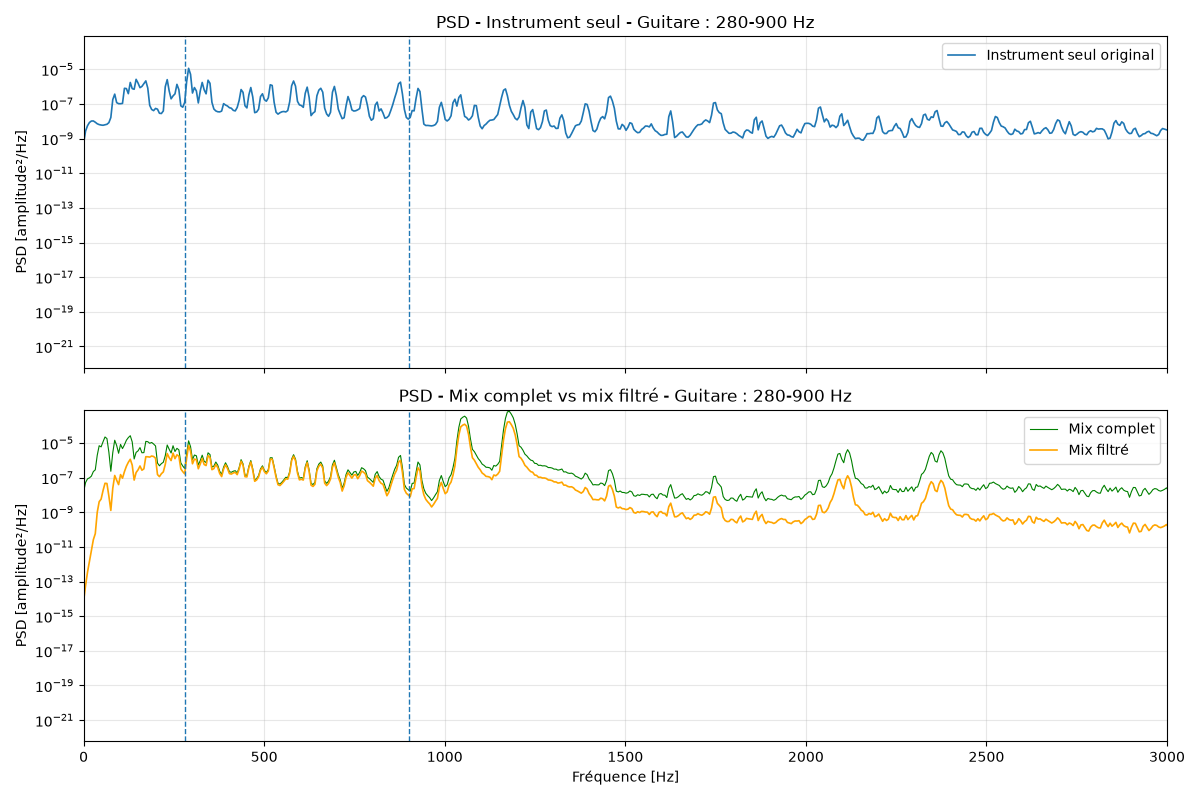
\includegraphics[width=\textwidth]{images/guitar_psd.png}
    \caption{Densité spectrale de puissance de la piste audio de la guitare}
    \label{fig:guitar_psd}
\end{figure}

\paragraph{Analyse des résultats de la flûte}

La FFT de la flûte seule (cf. figure \ref{fig:flute_fft}) montre que son énergie est concentrée dans une bande relativement étroite. Le signal filtré conserve correctement les composantes principales situées entre 1000 Hz et 1400 Hz. Cependant, certaines harmoniques situées au-dessus de 1500 Hz subsistent dans le mélange. Cela s'explique par les nombreuses harmoniques produites par la flûte mais également par les autres instruments. Le filtre réduit leur influence sans pouvoir les supprimer complètement. \\

La densité spectrale de puissance (cf. figure \ref{fig:flute_psd}) montre une forte réduction de puissance en dehors de la bande sélectionnée. En revanche, la puissance dans la bande 1000-1400 Hz reste très proche de celle observée sur le signal original. Cette observation confirme que le filtre conserve efficacement la partie utile du signal. \\

La séparation est nettement meilleure que pour la basse et la guitare électrique. Cela s'explique par le fait que la bande fréquentielle utilisée est moins encombrée par les autres instruments du mélange. \\

\begin{figure}
    \centering
    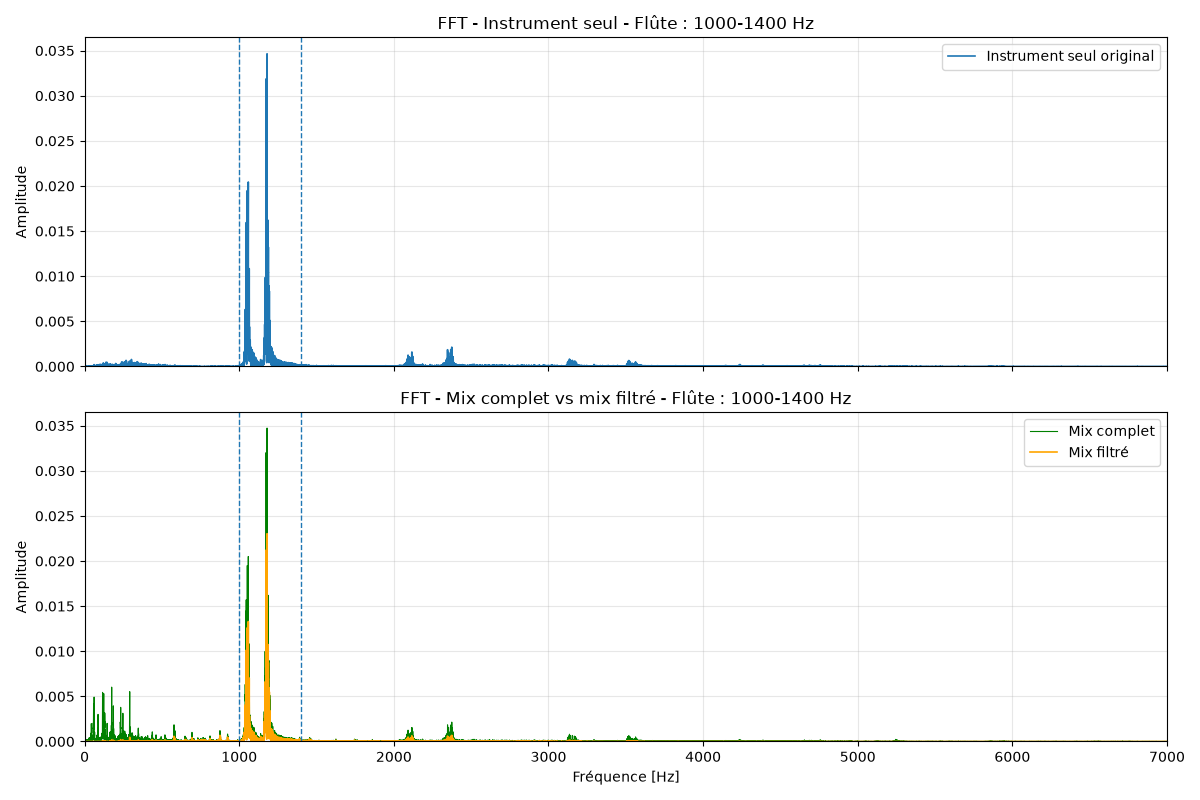
\includegraphics[width=\textwidth]{images/flute_fft.png}
    \caption{Spectre fréquentiel de la piste audio de la flûte}
    \label{fig:flute_fft}
\end{figure}

\begin{figure}
    \centering
    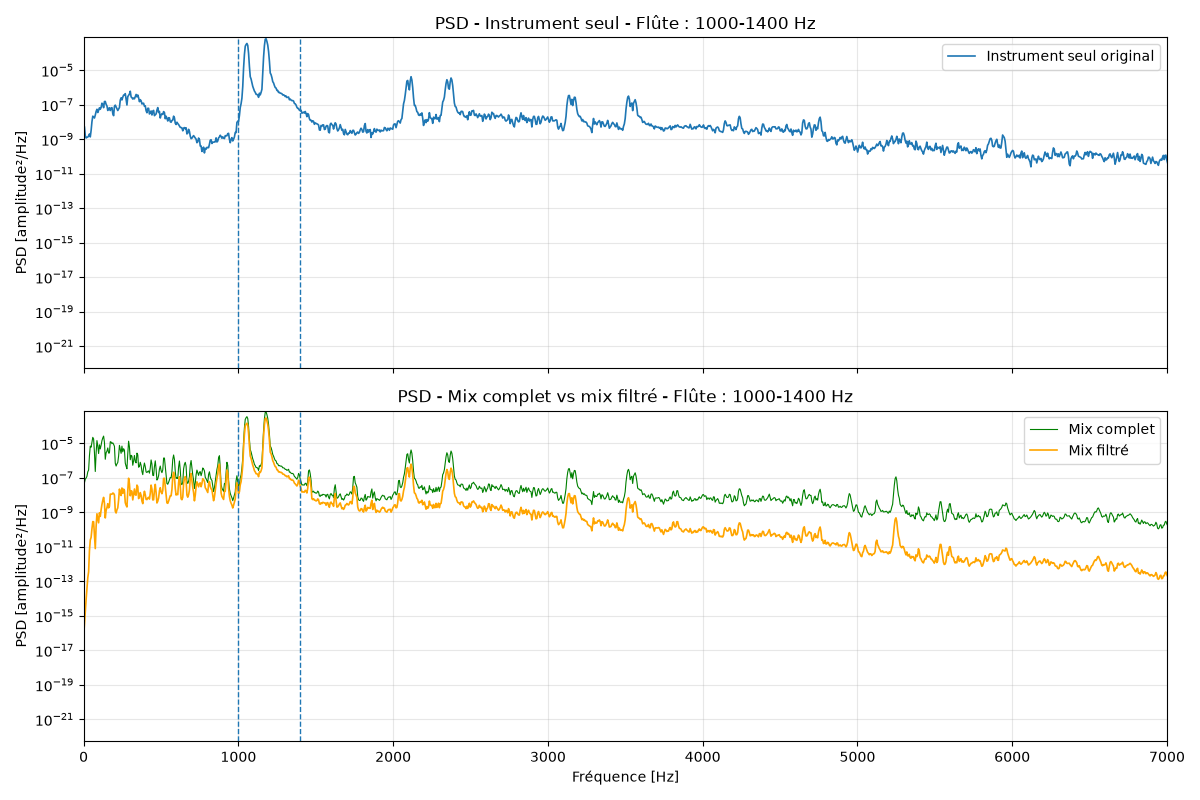
\includegraphics[width=\textwidth]{images/flute_psd.png}
    \caption{Densité spectrale de puissance de la piste audio de la flûte}
    \label{fig:flute_psd}
\end{figure}

\newpage

\paragraph{Analyse globale}
Avec les filtres passe-bas et passe-haut d'ordre 2, on a pu isoler les bandes fréquentielles caractéristiques de chaque instrument. Le filtrage a permis de réduire significativement les composantes indésirables provenant des autres instruments. Cependant, il est important de noter que certains résidus subsistent, en particulier pour la guitare électrique. Cela est dû aux harmoniques générées par les instruments et à la proximité des bandes fréquentielles. Une analyse plus approfondie pourrait être d'utiliser les données récupérées après filtrage et de recréer un signal audio pour écouter le résultat. \\
\FloatBarrier

\newpage